\section{Zielsetzung}

In dem Versuch V601 wird die Elektronenhülle eines Quecksilberatomes ($\ce{Hg}$)
untersucht. Das zugrunde liegende Ziel besteht aus der Überprüfung der Bohrschen
Postulate, die 1913 von Nils Bohr formuliert wurden.

\subsection{Hintergrund}

Der Franck-Hertz Versuch beschäftigt sich mit der Quantennatur der
Elektronenhülle eines Atomes. Dieser Versuch
ist nach den Physikern James Franck und Gustav Hertz benannt, die diesen
in den Jahren 1911-1914 ausarbeiteten und durchführten.

\section{Theorie}

Die Elektronenhülle lässt sich über Stoßexperimente erforschen. In dem
Franck-Hertz Versuch werden möglichst monoenergetische Elektronen
auf ein Quecksilbergas geschossen, sodass sie elastisch und unelastisch
mit den Atomgas stoßen.
Im Folgendem wird zuerst der schmatische Aufbau des Versuches dargestellt, da sich anhand
diesem die Gedankenzüge der Theorie verständlicher erläutern lassen.

\subsection{Schematischer Aufbau}

\begin{figure}
  \centering
  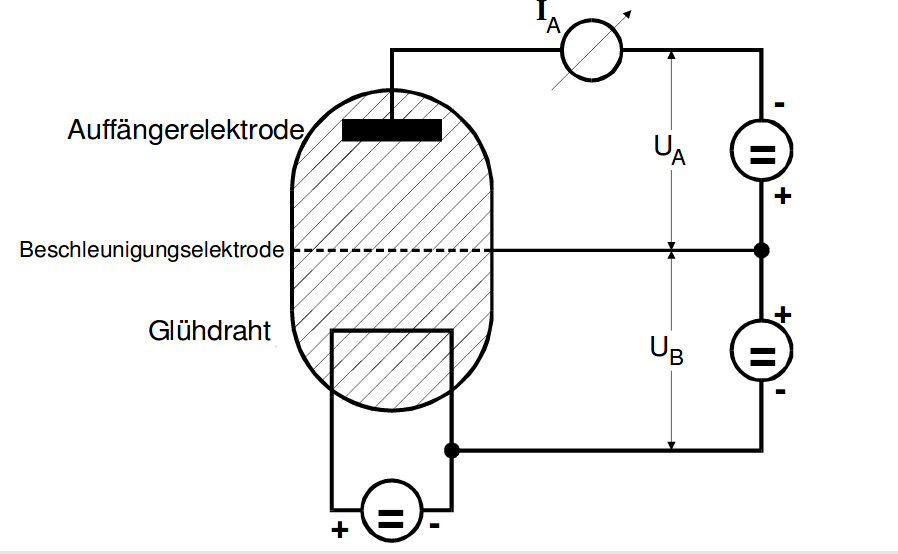
\includegraphics[width=9cm, height=5.5cm]{Pics/schematisch_Franck_Hertz.png}
  \caption{Schematischer Aufbau des Franck-Hertz Versuches.\cite{anleitung01}}
  \label{fig:schematisch_Franck_Hertz}
\end{figure}

Der schematische Aufbau ist in Abb. \ref{fig:schematisch_Franck_Hertz}
dargestellt.
Der schraffierte Bereich im Inneren des Gefäßes ist ein evakuierter Bereich, in dem sich
das $\ce{Hg}-$Gas befindet. Der Glühdraht stellt die Elektronenquelle für
die stoßenden Elektronen dar. Diese liegen aufgrund des Glühelektrischen-Effektes
als Elektronengas um den Glühdrah. Der Glühdraht dient als Kathode.
Die Beschleunigungselektrode ein von der Glühkathode verschiedenes Potential,
welches auf die Elektronen eine anziehende Kraft ausübt. Der Beschleunigungsdraht
dient somit als Anode. Zwischen den beiden erwähnten Elektroden liegt die
Spannung $\su{U}\ua{B}$ an.
Beschleunigte Elektronen nehmen auf der Beschleunigungsstrecke die Energie
$e_0 \cdot\su{U}\ua{B}$ in Form von kinetischer Energie auf.

Die beschleunigten Elektronen landen letztendlich auf der Auffängerelektrode.
Diese besitzt eine Bremsspannung $\su{U}\ua{A}$.
Nur Elektronen, die ausreichend kinietische Energie haben können dieses
Gegenfeld überwinden und an der Auffängerelektrode den Auffängerstrom $\su{I}\ua{A}$
verursachen. Dabei gilt die folgenden Energierelation.

\begin{equation}
  \label{eqn:Überwindungsenergie}
  \frac{m_0}{2}v_z^2 \geq e_0 \su{U}\ua{A}
\end{equation}

Die Elementarladung ist mit $e_0$ zu identifizieren.
Elektronen, die \eqref{eqn:Überwindungsenergie} erfüllen tragen zu
$\su{I}\ua{A}$ bei.

Der Energieverlust der Elektronen durch die Stöße wird mithilfe der Gegenfeldmessung
bestimmt. Das Gegenfeld ist in dem Aufbau \ref{fig:schematisch_Franck_Hertz}
durch die Bremsspannung $\su{U}\ua{A}$ realisiert.
Die Differenz zwischen Anfangsenergie und Endenergie spiegelt die
vom $\ce{Hg}$ aufgenommene Energie wieder.

Bohr postulierte, dass Elektronen nur auf diekreten Bahnen um den Atomkern bewege können.
Für den Franck-Hertz Versuch bedeutet dies, dass der Auffängerstrom
$\su{I}\ua{A}$ bei bestimmten Beschleunigungsspannungen abrupt abfällt.
Diese Energie ist genau dann erreicht, wenn die stoßenden Elektronen
die Quecksilberatome anregen. Der Ablauf ist schematisch wie folgt zu verstehen.

\begin{equation}
  \label{eqn:Reaktionsgleichung}
  \ce{(e^-)^* + Hg -> Hg^* + e^- -> Hg + e^- + \gamma}
\end{equation}

Dabei makiert $*$ die höher energetischen Zustände. Für das Elektronen
symbolisiert dies ein Zustand mit hoher kinetischer Energie.
$\ce{Hg^*}$ ist dabei der erste angeregte Zustand von Quecksilber.
Im ersten angeregten Zustand hat es eine Energie von $\su{E}_1$.
Nach dem angeregeten Zustand geht das $\ce{Hg^*}-$Atom nach einer
Relaxationszeit in der Größenordnung von $\SI{10e-8}{\second}$
unter Aussendung eines $\gamma-$Quantes in den Grundzustand über.
Im Grundzustand hat das Quecksilberatom eine Energie von $\su{E}_0$.
Der Lichtquant $\gamma$ hat eine Energie von

\begin{equation}
  \label{eqn:Lichtquant}
  h\nu = \su{E}_1 - \su{E}_0.
\end{equation}

$h$ ist das Planksche Wirkungsquantum und $\nu$ die Freqeunz des emitierten Lichtes.

Wird die Beschleunigungsspanung dem Auffängerstrom gegenüber aufgetragen
ergibt sich theoretisch die Kurve aus Abb. \ref{fig:Franck-Hertz-Kurve}.

\begin{figure}
  \centering
  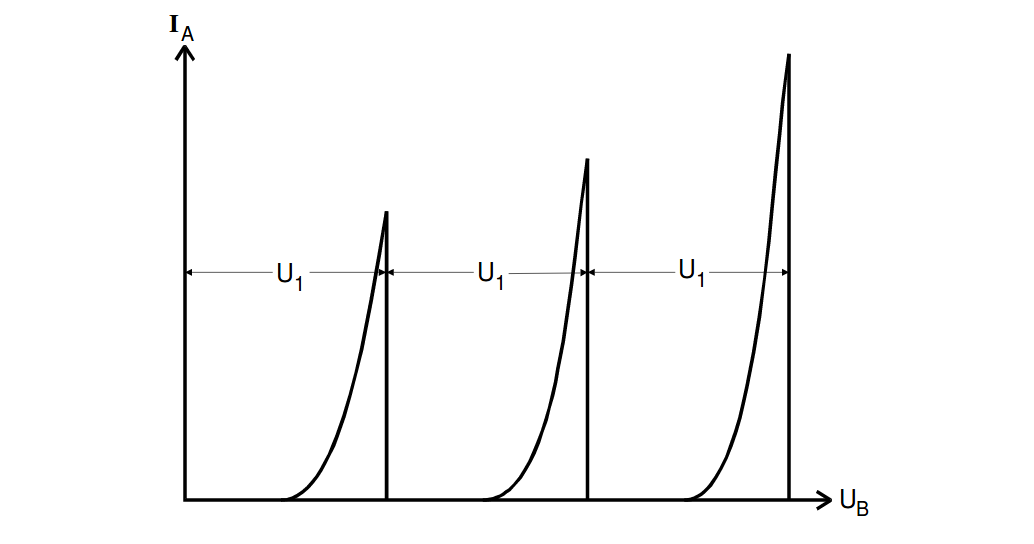
\includegraphics[width=\textwidth, height=7cm]{Pics/Franck_Hertz_Kurve.png}
  \caption{Theoretische Franck-Hertz-Kurve.\cite{anleitung01}}
  \label{fig:Franck-Hertz-Kurve}
\end{figure}

In den Bereichen in denen kein Auffängerstrom gemessen wird ist die
Energie der Elektronen nicht groß genug, um das Gegenfeld zu überwinden.
Mit steigender Beschleunigungsspannung werden mehr Elektronen von
dem Glühdraht angezogen. Deshalb nehmen die Maxima mit zunehmendem $\su{U}\ua{B}$
ebenfalls zu. Zudem sind die Maxima äquidistant auf der x-Achse angeordnet.
Die Abstände sind gleich dem ersten Anregungspotentials

\begin{equation}
  \label{eqn:Anregungspotential}
  \su{U}_1 = \frac{\left(\su{E}_1 - \su{E}_0\right)}{e_0}.
\end{equation}

Abbildung \ref{fig:Franck-Hertz-Kurve} stellt die idealisierte Franck-Hertz Kurve dar.
Die tatsächlich gemessene Kurve unterscheidet sich jedoch von der
Theoriekurve. Insgesamt sind vier Gründe für das Abweichen der theoretisch
von der praktisch bestimmten Franck-Hertz Kurve.
Zum Einen werden die Maxima der Franck-Hertz Kurve aufgrund des Kontaktpotentials
verschoben. Ein Kontaktpotential tritt auf, weil die Materialien des
Glühdrahtes und des Beschleinigungsdrahtes verschieden sind.
Das effektiv Beschleunigungspotential sieht wie folgt aus.

\begin{equation}
  \label{eqn:eff_Beschleunigungspot}
  \su{U}\ua{B, eff} = \su{U}\ua{B} - \frac{1}{e_0}\left(\su{\Phi}\ua{B} - \su{\Phi}\ua{G}\right)
\end{equation}

$\su{\Phi}\ua{B}$ ist dabei die Austrittsarbeit die für das Material des
Beschleunigungsdrahtes verwendet wird und $\su{\Phi}\ua{G}$ selbes für
den Glühdraht.
Der Verschiebungsfaktor der Maxima ist somit

\begin{equation}
  \label{eqn:Kontaktpotential}
  \su{K} = \frac{1}{e_0}\left(\su{\Phi}\ua{B} - \su{\Phi}\ua{G}\right).
\end{equation}

Dieser Ausdruck für $\su{K}$ wird Kontaktpotential genannt.

Desweiteren ist die Energieverteilung der Elektronen im Glühdraht nicht
monoenergetisch, wie in der Theorie angenommen wurde.
Es liegt eine kontinuierliche Energieverteilung vor, die durch die
Fermi-Dirac-Verteilung beschrieben wird. Damit ist die Geschwindigkeit der Elektronen
nach dem Austreten bereits $> 0$. Für die Franck-Hertz Kurve bedeutet das,
dass der Anstieg an die Maxima abgeflacht, im Vergleich zu der Idealkurve ist
und der abrupte Abfall nach dem Maxima nicht unstetig geschieht.

Zuzüglich wird die gemessene Kurve durch elastische Stöße im
Bereich zwischen der Beschleunigungselektrode und der Auffängerelektrode,
verglichen mit der Idealkurve
weiter abgeflacht. Auftretenden Richtungsänderungen,
hervorgerufen durch elastische Stöße führen auf eine Geschwindigkeitsverteilung
der z-Komponente der Elektronen. Das Ankommen der Elektronen auf der
Auffängerelektrode ist abhängig von der $\su{v}\ua{z}$-Komponente.

Der vierte Grund führ die Unterschiede zwischen der Ideal- und der gemessenen Kurve
hängt mit dem Einfluss des Dampfdruckes zusammen. Der Quecksilberdampf
wird in dem evakuierten Gefäß (vgl. Abb. \ref{fig:schematisch_Franck_Hertz})
durch spontan verdampfedes Quecksilber bereitgestellt.
Ein Tropfen Quecksilber ist in der Apparatur \ref{fig:schematisch_Franck_Hertz}
eingearbeitet. Gemäß der Dampfdruckkurve stellt sich ein Gleichgewichtsdampfdruck
$p\ua{sät}$ ein, der von der Umgebungstemperatur $\ua{T}$ abhängt.
Deshalb ist die mittlere freie Weglänge $\bar{w}$ ein entscheidender Faktor
des Versuches. $\bar{w}$ sollte klein im Vergleich zu dem Abstand $a$ zwischen
Kathode und Beschleunigungselektrode sein.
Die mittlere freie Weglänge hängt über

\begin{equation}
  \label{eqn:weglänge}
  \bar{w} [\su{cm}] = \frac{0,0029}{p\ua{sät}} [p \text{ in mbar}]
\end{equation}

mit dem Sättigungsdruck $p\ua{sät}$ zusammen. Es gibt einen Temperaturbereich,
in dem die Apparatur optimal arbeitet. Wird der Bereich deutlich unterschritten
ist die Stoßwahrscheinlichkeit zwischen $\ce{Hg}-$Atomen und Elektronen zu
gering. Die Franck-Hertz Kurve wäre dann die einhüllende der Idealkurve.
Hingegen ist bei zu hohen Temperaturen das Auftreten von elastischen Stößen
groß, sodass die Zahl der zu $\su{I}\ua{A}$ beitragen verringert ist. In diesem
Fall ist die Franck-Hertz Kurve gleich der Nullkurve.

\section{Durchführung}

\begin{figure}
  \centering
  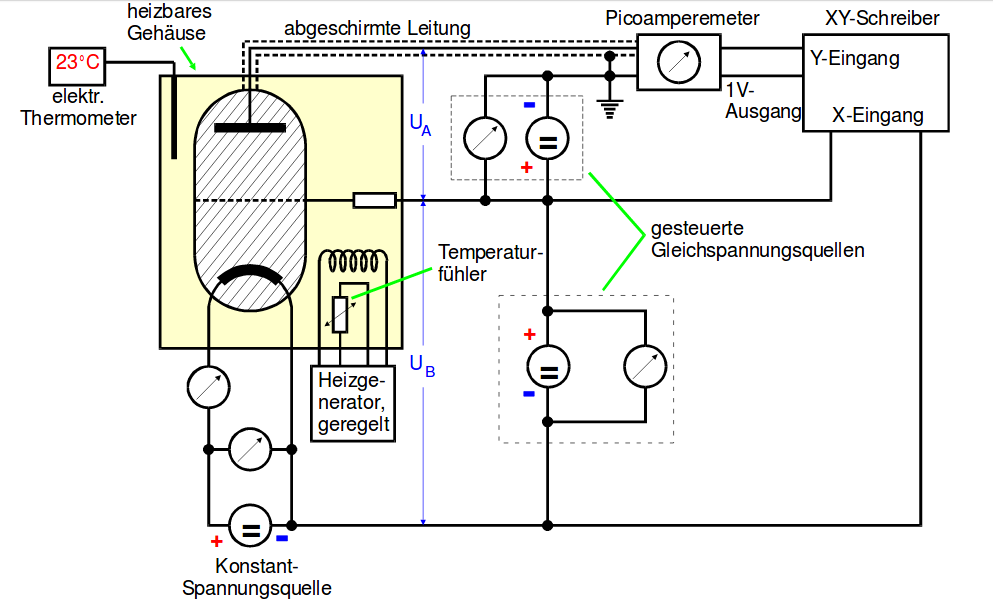
\includegraphics[width=\textwidth, height=8cm]{Pics/Aufbau.png}
  \caption{Theoretische Franck-Hertz-Kurve.\cite{anleitung01}}
  \label{fig:Aufbau}
\end{figure}

Mit dem Aufbau \ref{fig:Aufbau} wurde der Versuch durchgeführt.
Die Frank-Hertz-Apparatur ist in diesem integirert.
Der Auffängerstrom $\su{I}\ua{A}$ wird von dem Picoamperemeter gemessen.
Mithilfe des X-Y-Schreibers werden die die verschiedenen Messungen visualisiert.
An den Y-Kanal wird immer der Auffängerstrom $\su{I}\ua{A}$ den verschiedenen
Messungen entsprechend einer anderen Spannung gegenüber gestellt.
Der Heizgenerator kann manuell auf temperiert werden. Dieser dient dazu, die
Temperatur in dem Glaskolben aus Abb. \ref{fig:schematisch_Franck_Hertz}
variiren zu können. Die gesteuerten Gleichspannungsquellen dienen zur
Manipulation der Beschleunigungsspannung und der Auffängerspannung.
Die Gleichspannungsquellen können so eigestellt werden, dass sie
die Spannung über einen festgelegten Zeitraum konstant erhöhen oder
absenken können.

Zuerst ist die integrale Energieverteilung der beschleunigten Elektronen
zu bestimmen. Die Bremsspannung
$\su{U}\ua{A}$ wird auf den X-Kanal des Schreibers gelegt. Der Auffängerstrom
$\su{I}\ua{A}$ wird in Abhängigkeit von der Bremsspannung gemessen. Die
Beschleunigungsspannung $\su{U}\ua{B}$ ist währenddessen konstant auf
$\SI{11}{\volt}$ eingestellt.
Die Messung wird einmal bei Umgebungstemperatur und einmal bei
$T = \num{140} - \SI{160}{\celsius}$ durchgeführt.

Danach wird die Ionisierungsspannung $\su{U}\ua{ion}$ von Quecksilber bestimmt.
Dafür wird die Umgebungstemperatur auf $T = \num{100} - \SI{110}{\celsius}$ gereglet.
Die Bremsspannung wird nun konstant bei $\su{U}\ua{A} = \SI{-30}{\volt}$
gehalten. Der X-Kanal des XY-Schreibers wird mit der Beschleunigungsspanung
$\su{U}\ua{B}$ belegt, sodass der $\su{U}\ua{B}$ dem Auffängerstrom gegenüber
aufgetragen wird.

Abschließend ist die Temperatur auf $T = \num{160} - \SI{200}{\celsius}$ einzustellen.
Im Folgendem wird beschrieben, wie die Franck-Hertz Kurve aufgenommen wird.
Die Bremsspannung $\su{U}\ua{A}$ wird konstant bei $\SI{1}{\volt}$ gehalten und
die Beschleunigungsspannung durchläuft das Spannungsintervall von
$0 - 60\si{\volt}$. Die Bremsspannung ist an dem X-Kanal des
Schreibers angeschlossen und wird gegenüber des Auffängerstromes gemessen.
Die Temperatur ist zu variiren und es wird diejenige Kurve herangezogen, bei
der die Charakteristik der Franck-Hertz Kurve besonders deutlich werden.
Dabei sind Kurven mit vielen auftretenden Maxima zu bevorzugen.
